\documentclass[a4paper,10pt]{article}

%\usepackage{natbib}
\usepackage{amsthm}
\usepackage{amsfonts}
\usepackage{amssymb}
\usepackage{amsmath}
\usepackage{latexsym}
\usepackage{graphicx}
\usepackage{blindtext}

\usepackage{doc}

\newtheorem*{theorem}{Theorem}
\theoremstyle{definition}
\newtheorem*{definition}{Definition}

\hoffset -1in \topmargin 0mm \voffset 0mm \headheight 0mm
\headsep0mm
\oddsidemargin  20mm     %   Left margin on odd-numbered pages.
\evensidemargin 20mm     %   Left margin on even-numbered pages.
\textwidth   170mm       %   Width of text line.
\textheight  252mm

\makeatletter
\renewcommand\@openbib@code{%
     \advance\leftmargin  \z@ %\bibindent
      \itemindent \z@
     % Move bibitems close together
     \parsep -0.8ex
     }
\makeatother

\makeatletter
\renewcommand\section{\@startsection {section}{1}{\z@}%
                                   {-3.5ex \@plus -1ex \@minus -.2ex}%
                                   {1.5ex \@plus.2ex}%
                                   {\large\bfseries}}
\makeatother

\makeatletter
\renewcommand\subsection{\@startsection {subsection}{1}{\z@}%
                                   {-3.5ex \@plus -1ex \@minus -.2ex}%
                                   {1.5ex \@plus.2ex}%
                                   {\normalsize\bfseries}}
\makeatother

\makeatletter
	\setlength{\abovecaptionskip}{3pt}   % 0.25cm 
	\setlength{\belowcaptionskip}{3pt}   % 0.25cm 
\makeatother

\begin{document}
\pagestyle{empty}

\begin{center}
{\bf \Large Snake-like robots}
\end{center}

\smallskip
\begin{center}
{\large Tran Duc Viet}
\end{center}

\smallskip
\begin{center}
Faculty of Mechanical Engineering, Brno University of Technology\\
Institute of Automation and Computer Science\\
Technická 2896/2, Brno 616 69, Czech Republic\\
192028@vutbr.cz\\
\end{center}

\bigskip
\noindent Abstract: \textit{This short seminar work deals with short intorooduction to snake.like locomotion and snake-like robots.}

\vspace*{10pt} \noindent Keywords: \textit{Snake-like locomotion, snake-like robot.}

\bigskip
\section{Introduction}
\label{sec:1}
Robotics is rather new field which, without doubt, has endless potential. Skipping the origin of the word “robot”, important figures in this field, or even the first full-fledged robot to ever exist, this short seminar work focuses on bio-inspired robots, specifically snake-like robots.

First let us thinks about why do people even create robots. There are many various reasons, one of the surely is that the robot meant to help people with labour. It is meant to do the work, which would otherwise be very exhausting, or maybe even impossible for a person to do. It is meant to replace the person in the specific activity. It is certain, that the replacement should be at least as good as the original, if not even better. From a certain perspective, it is the replacement trying to imitate the original and at this point we may say that the fake was inspired by the original, whatever that original might be.


\section{Snake-like locomotion}
In order to imitate the movements of the original, one must first take a closer look the structure of said original. Living snakes are interesting choice for the robot-maker enthusiasts due to their unique anatomy. The aim of this work is not to dig deep into biology, but in short - their bodies consist basically of a long spine and numerous ribs with various muscles in between. What is more interesting are the movements that have been observed and further studied. Today we recognize 4 main types.

\subsection{Rectilinear locomotion}
This type of locomotion is typical for bigger snakes. The trick is in utilizing the abdominal scales and abdominal muscles. This method allows motion in direct path and can be compared to crawler; however, this method somewhat lacks in terms of speed compared to other methods. [1] [2] [3]
\begin{figure}[h!]
\begin{center}
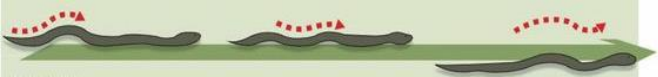
\includegraphics[scale=0.75]{image/Rectilinear_locomotion.png}
\caption{Rectilinear undulation [4]}
\label{fig:1}
\end{center}
\end{figure}

\vspace*{100pt}

\subsection{Lateral undulation}
Sometimes called serpentina motion, this method is the most common among the snakes. The method is highly efficient in rocky or similar environments, where various protrusions are abundant. [1] [2] [3]
\begin{figure}[h!]
\begin{center}
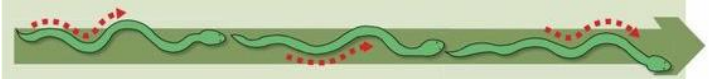
\includegraphics[scale=0.75]{image/Lateral_undulation.png}
\caption{Lateral undulation [4]}
\label{fig:2}
\end{center}
\end{figure}

\subsection{Concertina locomotion}
This locomotion consists of series of contracting and “shooting” the snake’s body. While this method offers low traveling speed, it is sometimes necessary. It might be useful for example jumping between tree branches or hunting in burrows. [1] [2] [3]
\begin{figure}[h!]
\begin{center}
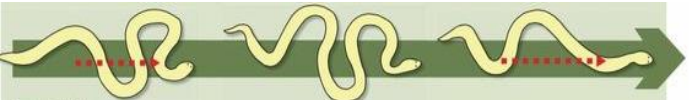
\includegraphics[scale=0.75]{image/Concertina_locomotion.png}
\caption{Concertina locomotion [4]}
\label{fig:}
\end{center}
\end{figure}

\subsection{Sidewinding}
This type is unique and is used by snakes living in sandy environment, where any other methods would prove inefficient due to lack of solid support on the surface.
\begin{figure}[h!]
\begin{center}
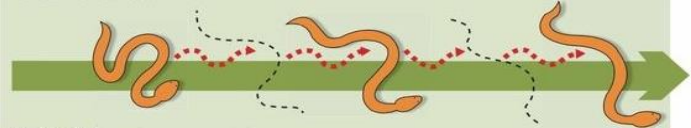
\includegraphics[scale=0.75]{image/Sidewinding.png}
\caption{Sidewinding [4]}
\label{fig:4}
\end{center}
\end{figure}

\section{Snake-like robots}
There are plentiful snake-like robots nowadays and many more are in development in the present. There are differences, be it overall construction, motion method or even power unit. One of the dominant figures in this field Tokyo Institute of Technology classifies all their concepts into 5 base categories. There are few examples listed in each category.
\begin{figure}[h!]
\begin{center}
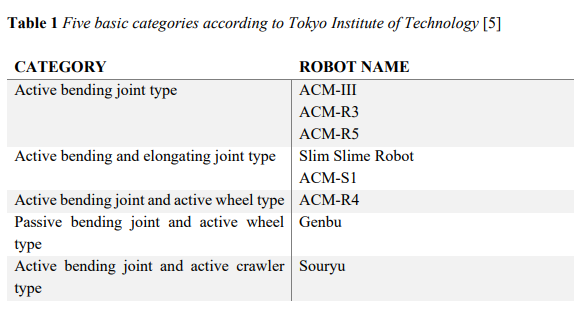
\includegraphics[scale=0.75]{image/Categories.png}
\label{}
\end{center}
\end{figure}

\vspace*{50pt}

\subsection{Active bending joint type}
ACM-III (Active Cord Mechanism – III)

One of the first to ever mathematically describe snake-like locomotion was 
J. Gray in his works in 1946. Japanese professor Hirose Shigeo followed up and 
in 1972 he introduced ACM-III model, which is dubbed as the first snake-like 
robot to ever successfully demonstrate snake-like locomotion. [5] [6]
\begin{figure}[h!]
\begin{center}
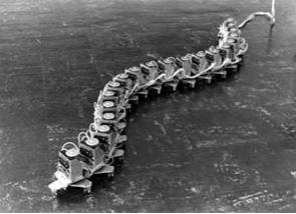
\includegraphics[scale=0.75]{image/ACM-III.png}
\caption{ACM-III [6]}
\label{}
\end{center}
\end{figure}

\newpage

\subsection{Active bending joint and elongating joint type}
Slim Slime Robot

The model consists of linearly connecting multiple modules that 
pneumatically bend and elongate. The robot was designed for manoeuvring in 
long, narrow pipes. [5] [6]
\begin{figure}[h!]
\begin{center}
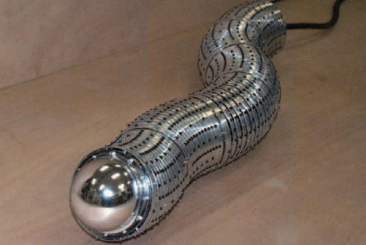
\includegraphics[scale=0.75]{image/Slim_slime_robot.png}
\caption{Slim slime robot [6]}
\label{}
\end{center}
\end{figure}

\subsection{Active bending joint and active wheel type}
ACM-R4(Active Cord Mechanism-R4)

This model is basically modification of previous model ACM-R3, which 
belongs to the 1st category. While the ACM-R3 added just the possibility of 3D 
movement, all movements were just results of bending joints in various patterns. 
ACM-R4 however has active wheel which further improves overall mobility. [5] 
[6]

\begin{figure}[h!]
\begin{center}
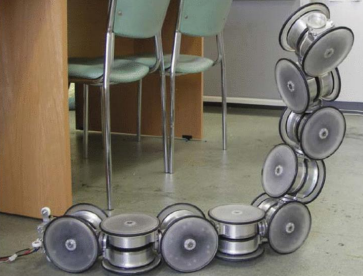
\includegraphics[scale=0.75]{image/ACM-R4.png}
\caption{ACM-R4 [6]}
\label{}
\end{center}
\end{figure}

\subsection{Passive bending joint and active wheel type}
Genbu

As the name of the category suggests, the movement is assured mainly by 
active wheels, therefore is only natural, that the attention should be focused of 
said part of the robot. The Genbu model was designed to have dominant wheels 
and joints to passively provide better grip of the surface. [5] [6]

\begin{figure}[h!]
\begin{center}
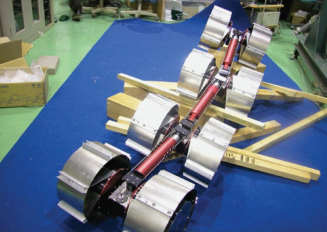
\includegraphics[scale=0.75]{image/Genbu.png}
\caption{Genbu [6]}
\label{}
\end{center}
\end{figure}

\vspace*{60pt}

\subsection{Active bending joint and active crawler type}
Souryu

The Souryu series was developed with the desire to be able to move in extreme 
environment caused by natural disasters. The following figure shows Souryu-IV 
which consists of 3 segments each possessing a crawler. The segments are 
connected via rods which allows slight rotation. [5] [6]

\begin{figure}[h!]
\begin{center}
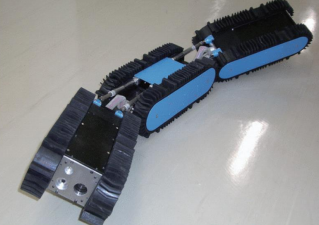
\includegraphics[scale=0.75]{image/Souryu-IV.png}
\caption{Souryu-IV [6]}
\label{}
\end{center}
\end{figure}

\section{Snake-like robot application}
Many research groups around the world have various goals. There is one goal that almost 
every group more or less tries to achieve – that is to deploy the robot into the environment 
where all conventional equipment fails. An example would be sites struck by natural 
disaster, where all movement would be restricted due to debris and unknown dangers.

September 2017 central Mexico was struck by an M 7.1 earthquake which lasted 
20 second, claiming almost 400 lives and injuring over 6000, making it the second worst 
earthquake of the year. [7] Help from all corners around the world arrived in many forms 
be it volunteer rescue units, donations, or equipment. Among many, the Carnegie Mellon 
University from Pittsburgh also contributed with a snake-like robot and a team of 
operators. The team actively participated in rescue activities in Mexico City, by deploying 
the robot to two different passages the snakebot was able to provide rescue workers with 
the feed through the debris, unfortunately without success. Still, the mission provided 
valuable experience in demonstrating the robot’s capabilities in an actual rescue mission.
The snake robot received positive reactions from on-site rescue personnel and Mexican 
Red Cross even expressed their desire to own such robot in the future.[8]

\begin{figure}[h]
\begin{center}
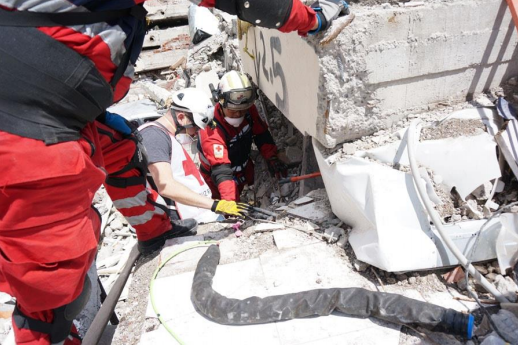
\includegraphics[scale=0.75]{image/Rescue_mission_in_Mexico_City.png}
\caption{Rescue mission in Mexico City [8]}
\label{}
\end{center}
\end{figure}

\section{Conclusion}
Snake-like robots have endless potential and can be applied in almost every thinkable 
field. Be it scouting dangerous or inaccessible areas as a rescue bot or performing 
surgeries requiring extreme precision, it all comes down to ability to perform desired 
movements. Thanks to the snake-like shape, the choice of possible movement is 
practically endless.

Even though we may find snake-like robot in here and there today, the true 
utilization of their potential is yet to be achieved. It is rather experimental, and not very 
common; however, the overall progress is undeniable, and it is just matter of time when
the snakebots will be truly relied upon.

\newpage
\section{References}
\begin{figure}[h]
\begin{center}
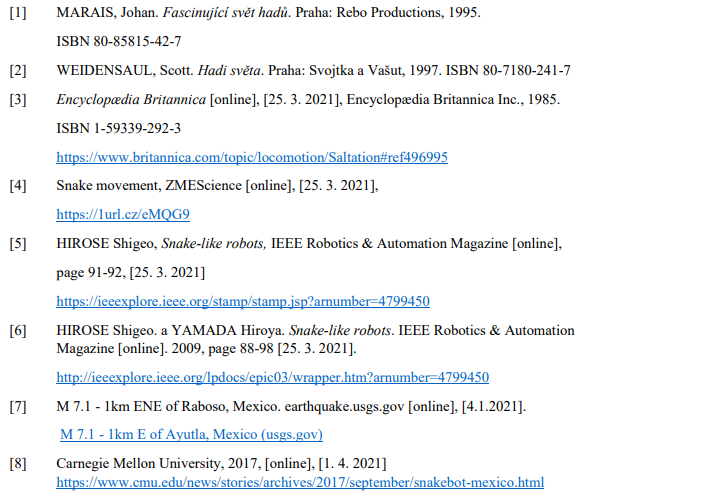
\includegraphics[scale=1]{image/References.png}
\label{}
\end{center}
\end{figure}


%Figures\footnote{If you copy text passages, figures, or tables from other works, you must obtain \textit{permission} from the copyright holder (usually the original publisher or author). Please enclose the signed permission with the manuscript.} and tables should be numbered as follows: Fig.~1,
%Fig.~2,\,\dots{} etc. (see Fig.~\ref{fig:1}), Table 1, Table 2,\,\dots{} etc. (see Table~\ref{tab:1}). Figure caption must be placed below the figure and table caption must be placed above the table.
%Some reference \cite{SICILIANO_rhandbook}.

% References
%
%\begingroup
%\makeatletter
%\renewcommand\section{\@startsection {section}{1}{\z@}%
%                                   {-3.5ex \@plus -1ex \@minus -.2ex}%
%                                {4.5ex \@plus.2ex}%
%                                   {\large\bfseries}}
%\makeatother


%\bibliography{references}{}
%\bibliographystyle{acm}
%\endgroup

\end{document}